\chapter{A/A WEAPONS}
\thumbtab{A/A}{5}
\minitoc
\cleardoublepage

\section{M61 GUN}
\subsection{M61 GUN - OVERVIEW}
\begin{tableitemize}
    \blueitem{GUN RATE \break Button}{
    \begin{subitemize}
        \item \textbf{Cycles Gun Rate}
        \begin{itemize}
            \item \textbf{HIGH} -- 6000 rpm
            \item \textbf{LOW} -- 4000 rpm
        \end{itemize}
    \end{subitemize}}
    \blueitem{A/A Gun Modes}{
    \begin{subitemize}
        \item \textbf{RTGS} -- \textbf{R}eal-\textbf{T}ime \textbf{G}un\textbf{S}ight Mode
        \begin{itemize}
            \item Selected automatically with guns
            \item \textbf{If No WCS Data Available} displays bullet location at 2000 ft with diamond and 1000 ft with pipper
            \item \textbf{If WCS Data Available} pipper displays bullet location at targets current range out to 4000 ft
        \end{itemize}
        \item \textbf{MANUAL}
        \begin{itemize}
            \item Fixed manual pipper
            \item Adjust with \textbf{GUN ELEV} knob
            \item Press \textbf{CAGE/SEAM} to select
        \end{itemize}
    \end{subitemize}}
    \blueitem{CAGE/SEAM \break Button}{
    \begin{subitemize}
        \item \textbf{Cycles RTGS / MANUAL Gun Modes}
    \end{subitemize}}
    \blueitem{ROUNDS Knob}{
    \begin{subitemize}
        \item \textbf{Allows selection of remaining gun rounds}
    \end{subitemize}}
\end{tableitemize}

\clearpage

\subsection{M61 GUN - MANUAL}
\begin{tablenumerate}
    \blueitem{Pilot Conditions}{		
    \begin{subitemize}
        \item \textbf{MASTER ARM} \dotfill \textbf{ON}
        \item \textbf{HUD} \dotfill \textbf{A/A}
        \item \textbf{Gun Rate} \dotfill \textbf{HIGH}
        \item \textbf{Gunsight Lead} \dotfill as required
        \item \textbf{WEAPON SELECTOR} \dotfill \textbf{GUNS}
    \end{subitemize}}
    \blueitem{Employment}{		
    \begin{subenumerate}
        \item \textbf{Gun Mode} \dotfill \textbf{MANUAL}
        \item \textbf{Pipper} \dotfill on target
        \item \textbf{Trigger} \dotfill \textbf{FIRE}
    \end{subenumerate}}
\end{tablenumerate}

\subsection{M61 GUN - RTGS /  NO RADAR}
\begin{tablenumerate}
    \blueitem{Pilot Conditions}{		
    \begin{subitemize}
        \item \textbf{MASTER ARM} \dotfill \textbf{ON}
        \item \textbf{HUD} \dotfill \textbf{A/A}
        \item \textbf{Gun Rate} \dotfill \textbf{HIGH}
        \item \textbf{WEAPON SELECTOR} \dotfill \textbf{GUNS}
    \end{subitemize}}
    \blueitem{Employment}{		
    \begin{subenumerate}
        \item \textbf{Gun Mode} \dotfill \textbf{RTGS}
        \item \textbf{Pipper} \dotfill on target
        \item \textbf{Trigger} \dotfill \textbf{FIRE}
    \end{subenumerate}}
\end{tablenumerate}

\subsection{M61 GUN - RTGS / RADAR}
\begin{tablenumerate}
    \blueitem{Pilot Conditions}{		
    \begin{subitemize}
        \item \textbf{MASTER ARM} \dotfill \textbf{ON}
        \item \textbf{HUD} \dotfill \textbf{A/A}
        \item \textbf{Gun Rate} \dotfill \textbf{HIGH}
        \item \textbf{WEAPON SELECTOR} \dotfill \textbf{GUNS}
    \end{subitemize}}
    \blueitem{Employment}{		
    \begin{subenumerate}
        \item \textbf{Gun Mode} \dotfill \textbf{RTGS}
        \item \textbf{Radar} \dotfill \textbf{STT}
        \item \textbf{Pipper} \dotfill on target
        \item \textbf{Trigger} \dotfill \textbf{FIRE}
    \end{subenumerate}}
\end{tablenumerate}

\clearpage
\section{AIM-9 SIDEWINDER}
\subsection{AIM-9 - OVERVIEW}
\begin{tableitemize}
    \blueitem{Missile \break Preparation}{
    \begin{subitemize}
        \item \textbf{MSL PREP}
        \begin{itemize}
            \item AIM-9 seeker must be cooled
            \item Either press \textbf{SW COOL} button
            \item Or activation of \textbf{ACM}
        \end{itemize}
    \end{subitemize}}
    \blueitem{Seeker Head Modes}{
    \begin{subitemize}
        \item \textbf{SEAM} -- \textbf{S}idewinder \textbf{E}xpanded \textbf{A}cq. \textbf{M}ode
        \begin{itemize}
            \item \textbf{Double-D} search pattern (invisible to pilot)
            \item 4.5 sec search time
            \item Allows AIM-9 to uncage \& track target
            \item 40 deg track limit
            \item WCS slaves AIM-9 to radar track
        \end{itemize}
        \item \textbf{Boresight}
        \begin{itemize}
            \item AIM-9 locked to ADL
            \item 2.5 deg FOV
            \item Selected if  \textbf{MODE/STP} set to \textbf{BRSIT}
            (and \textbf{ACM} not active)
        \end{itemize}
    \end{subitemize}}
    \blueitem{MODE/STP \break Switch}{
    \begin{subitemize}
        \item \textbf{NORM}
        \begin{itemize}
            \item Allows \textbf{SEAM} seeker mode
        \end{itemize}
        \item \textbf{BRSIT}
        \begin{itemize}
            \item Forces Boresight seeker mode
            \item Overridden if \textbf{ACM} active
        \end{itemize}
    \end{subitemize}}
    \blueitem{CAGE/SEAM \break Button}{
    \begin{subitemize}
        \item \textbf{Uncages Seeker}
        \begin{itemize}
            \item Starts 4.5 second double-D search
            \item If no IR source found cages again
        \end{itemize}
        \item \textbf{Slaves Seeker}
        \begin{itemize}
            \item If radar STT locked
        \end{itemize}
    \end{subitemize}}
\end{tableitemize}

\clearpage

\subsection{AIM-9 - SILENT}
\begin{tablenumerate}
    \blueitem{Pilot Conditions}{		
    \begin{subitemize}
        \item \textbf{MASTER ARM} \dotfill \textbf{ON}
        \item \textbf{HUD} \dotfill \textbf{A/A}
        \item \textbf{SW COOL} \dotfill \textbf{ON}
        \item \textbf{MODE/STP} \dotfill \textbf{As Desired}
        \item \textbf{WEAPON SELECTOR} \dotfill \textbf{SW}
    \end{subitemize}}
    \blueitem{Employment}{		
    \begin{subenumerate}
        \item \textbf{CAGE/SEAM} \dotfill \textbf{Uncage Seeker}
        \item \textbf{IR-Lock} \dotfill \textbf{Good Tone}
        \item \textbf{Trigger} \dotfill \textbf{FIRE}
    \end{subenumerate}}
\end{tablenumerate}

\subsection{AIM-9 - RADAR}
\begin{tablenumerate}
    \blueitem{Pilot Conditions}{		
    \begin{subitemize}
        \item \textbf{MASTER ARM} \dotfill \textbf{ON}
        \item \textbf{HUD} \dotfill \textbf{A/A}
        \item \textbf{SW COOL} \dotfill \textbf{ON}
        \item \textbf{MODE/STP} \dotfill \textbf{NORM}
        \item \textbf{WEAPON SELECTOR} \dotfill \textbf{SW}
    \end{subitemize}}
    \blueitem{Employment}{		
    \begin{subenumerate}
        \item \textbf{Radar} \dotfill \textbf{STT}
        \item \textbf{CAGE/SEAM} \dotfill \textbf{Slave Seeker}
        \item \textbf{IR-LOCK} \dotfill \textbf{Good Tone}
        \item \textbf{Steering} \dotfill center T-shaped cue with ASE
        \item \textbf{Trigger} \dotfill \textbf{FIRE}
    \end{subenumerate}}
\end{tablenumerate}

\clearpage

\section{AIM-7 SPARROW}
\subsection{AIM-7 - OVERVIEW}
\begin{tableitemize}
    \blueitem{Missile \break Preparation}{
    \begin{subitemize}
        \item \textbf{MSL PREP}
        \begin{itemize}
            \item AIM-7 must be tuned to AWG-9
            \item Either press \textbf{MSL PREP} button
            \item Or activation of \textbf{ACM}
        \end{itemize}
    \end{subitemize}}
    \blueitem{Launch Modes}{
    \begin{subitemize}
        \item \textbf{Normal}
        \begin{itemize}
            \item Standard operation, STT target designated before launch
            \item AIM-7 uses SARH all the way to target
            \item WCS can use CS or PD for guidance set with \textbf{MSL OPTIONS} Switch
        \end{itemize}
        \item \textbf{Boresight}
        \begin{itemize}
            \item Uses CW flood antenna of AWG-9
            \item Missile will \textbf{track strongest return} in Flood area
            \item Automatically activated if STT broken
            \item Selected if \textbf{MODE/STP} set to \textbf{BRSIT}
            \item \textbf{Or if no STT available}
            \item \textbf{Shown Below}
        \end{itemize}
    \end{subitemize}}
    \blueitem{MSL SPD  \break  GATE Switch}{
    \begin{subitemize}
        \item \textbf{NOSE QTR}
        \begin{itemize}
            \item Standard setting in DCS
        \end{itemize}
        \item \textbf{All Others}
        \begin{itemize}
            \item Not simulated
        \end{itemize}
    \end{subitemize}}
    \blueitem{MSL OPTIONS  \break  Switch}{
    \begin{subitemize}
        \item \textbf{NORM}
        \begin{itemize}
            \item WCS uses dedicated CW antenna for AIM-7 guidance
        \end{itemize}
        \item \textbf{SP PD}
        \begin{itemize}
            \item WCS uses PD from main flood antenna for AIM-7F/M guidance
        \end{itemize}
    \end{subitemize}}
    \blueitem{MODE/STP \break Switch}{
    \begin{subitemize}
        \item \textbf{NORM}
        \begin{itemize}
            \item Sets normal launch mode logic
        \end{itemize}
        \item \textbf{BRSIT}
        \begin{itemize}
            \item Forces Boresight launch mode
        \end{itemize}
    \end{subitemize}}
\end{tableitemize}

\begin{figure}[htbp]
    \centering
    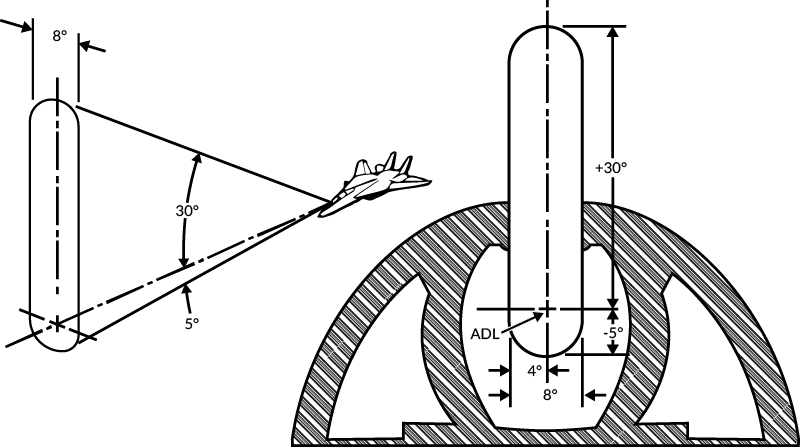
\includegraphics[width=0.9\linewidth]{cwflood.png}
    \caption{\textbf{CW Flood Search Pattern}}
    \label{fig:cwflood}
\end{figure}

\subsection{AIM-7 - STT}
\begin{tablenumerate}
    \blueitem{Pilot Conditions}{		
    \begin{subitemize}
        \item \textbf{MASTER ARM} \dotfill \textbf{ON}
        \item \textbf{HUD} \dotfill \textbf{A/A}
        \item \textbf{MSL PREP} \dotfill \textbf{ON}
        \item \textbf{MODE/STP} \dotfill \textbf{NORM}
        \item \textbf{WEAPON SELECTOR} \dotfill \textbf{SP}
    \end{subitemize}}
    \dblueitem{RIO Conditions}{		
    \begin{subitemize}
        \item \textbf{MSL SPD GATE} \dotfill \textbf{NOSE QTR}
        \item \textbf{MSL OPTIONS} \dotfill \textbf{As Desired}
    \end{subitemize}}
    \blueitem{Employment}{		
    \begin{subenumerate}
        \item \textbf{Radar} \dotfill \textbf{STT}
        \item \textbf{Steering}
        \begin{itemize}
            \item \textbf{Target} < 20 deg from ADL
            \item \textbf{ASE} center T-shaped cue within
        \end{itemize}
        \item \textbf{Trigger} \dotfill \textbf{Press and Hold} \\
        \hfill (until weapon release)
        \item \textbf{Radar} \dotfill \textbf{Maintain Lock} \\
        \hfill (until impact)
    \end{subenumerate}}
\end{tablenumerate}

\clearpage

\subsection{AIM-7 - PDSTT -VS- PSTT}
\begin{tableitemize}
    \blueitem{PSTT}{
    \begin{subitemize}
        \item \textbf{AIM-7 Guided in CW Mode}
        \item \textbf{PSTT Advantages / Disadvantages}
        \begin{itemize}
            \item Susceptable to ground clutter 
            \item In close range scenarios (<20 NM) extremely hard to break lock
        \end{itemize}
    \end{subitemize}}
    \blueitem{PDSTT}{
    \begin{subitemize}
        \item \textbf{AIM-7 CAN be Guided in SP PD Mode}
        \begin{itemize}
            \item Requires \textbf{MSL OPTIONS} -- \textbf{SP PD}
            \item Only available on AIM-7F and newer
        \end{itemize}
        \item \textbf{PDSTT Advantages / Disadvantages}
        \begin{itemize}
            \item Susceptable to notching
            \item Enables longest range Sparrow shots
        \end{itemize}
    \end{subitemize}}
\end{tableitemize}

\notebox{
    \begin{itemize}
        \item \textbf{If launch is initiated on a PDSTT target with MSL OPTIONS switch set to NORM}
        \begin{itemize}
            \item CW illumination \& guidance will be used
            \item Lock still based off PDSTT
        \end{itemize}
    \end{itemize}
}

\clearpage

\section{AIM-54 PHOENIX}
\subsection{AIM-54 - OVERVIEW}
\begin{tableitemize}
    \blueitem{Missile \break Preparation}{
    \begin{subitemize}
        \item \textbf{Weapon Cooling}
        \begin{itemize}
            \item AIM-54 requires liquid cooling
            \item RIO enabled \textbf{LIQUID COOLING} switch
        \end{itemize}
        \item \textbf{MSL PREP}
        \begin{itemize}
            \item AIM-54 must be tuned to AWG-9
            \item Either press \textbf{MSL PREP} button
            \item Or activation of \textbf{ACM}
        \end{itemize}
    \end{subitemize}}
    \blueitem{Launch Modes}{
    \begin{subitemize}
        \item \textbf{PDSTT SARH}
        \begin{itemize}
            \item AIM-54 uses SARH all the way to target
            \item Faster update rate than TWS
            \item \textbf{Slightly increased effective range} as compared to a TWS launch
        \end{itemize}
        \item \textbf{TWS SARH/ARH}
        \begin{itemize}
            \item Allows \textbf{6 launches at 6 targets}
            \item Missile initially SARH guided
            \item When within AIM-54 seeker range AWG-9 sends activation command
            \item \textbf{Not Fire and Forget:} Requires automatic activation command
        \end{itemize}
        \item \textbf{ACM Active}
        \begin{itemize}
            \item Activated when \textbf{BRSIT} selected
            \item Or \textbf{ACM} active with no radar track
            \item Missile commanded active \textbf{before launch}
        \end{itemize}
    \end{subitemize}}
    \blueitem{MSL SPD  \break  GATE Switch}{
    \begin{subitemize}
        \item \textbf{NOSE QTR} -- Standard setting in DCS
        \item \textbf{All Others} -- Not simulated
    \end{subitemize}}
    \blueitem{MSL OPTIONS  \break  Switch}{
    \begin{subitemize}
        \item \textbf{NORM}
        \begin{itemize}
            \item Normal guidance (SARH or SARH/ARH)
        \end{itemize}
        \item \textbf{PH ACT}
        \begin{itemize}
            \item WCS immediately sends AIM-54 activation command on launch
            \item Reverts to SARH if no target detected
            \item \textbf{Must be selected before launch}
        \end{itemize}
    \end{subitemize}}
    \blueitem{TGTS  \break  Switch}{
    \begin{subitemize}
        \item \textbf{SMALL} -- 6nm activation range
        \item \textbf{NORM} -- 10nm activation range
        \item \textbf{LARGE} -- 13nm activation range
    \end{subitemize}}
    \blueitem{Missile Next  \break  Launch Button}{
    \begin{subitemize}
        \item \textbf{Selects Hooked Track as Next Target for AIM-54 TWS Engagement}
    \end{subitemize}}
    \blueitem{MODE/STP \break Switch}{
    \begin{subitemize}
        \item \textbf{NORM} -- Normal operation
        \item \textbf{BRSIT}
        \begin{itemize}
            \item Commanded active \textbf{before launch}
            \item Missile follows ADL and locks strongest return
        \end{itemize}
    \end{subitemize}}
    \blueitem{TWS Symbology}{
    \hyperref[subsec:tidsymb]{\textbf{Refer to TID Symbology Section}}
    \begin{subitemize}
        \item \textbf{Pre-Launch}
        \begin{itemize}
            \item Prioritization numbers assigned to tracks automatically or manually
            \item Blinking indicates optimal launch parameters
        \end{itemize}
        \item \textbf{Post-Launch}
        \begin{itemize}
            \item Target prioritization number replaced with TTI
            \item Other prioritization numbers collapsed by one
            \item Tracks under missile attack brightened
            \item \textbf{TTI blinks when missile active}
        \end{itemize}
    \end{subitemize}}
    \blueitem{Launch To Eject (LTE) Time}{
    \begin{subitemize}
        \item \textbf{Normal Operation} -- 3-4 seconds
        \item \textbf{When in ACM} -- 1 second
    \end{subitemize}}
\end{tableitemize}

\clearpage

\subsection{AIM-54 - PD-STT}
\begin{tablenumerate}
    \blueitem{Pilot Conditions}{
    \begin{subitemize}
        \item \textbf{MASTER ARM} \dotfill \textbf{ON}
        \item \textbf{HUD} \dotfill \textbf{A/A}
        \item \textbf{MSL PREP} \dotfill \textbf{ON}
        \item \textbf{MODE/STP} \dotfill \textbf{NORM}
        \item \textbf{WEAPON SELECTOR} \dotfill \textbf{PH}
    \end{subitemize}}
    \dblueitem{RIO Conditions}{		
    \begin{subitemize}
        \item \textbf{LIQUID COOLING} \dotfill \textbf{ON (FWD)}
        \item \textbf{MSL SPD GATE} \dotfill \textbf{NOSE QTR}
        \item \textbf{MSL OPTIONS} \dotfill \textbf{As Desired}
        \item \textbf{TGTS Switch} \dotfill \textbf{As Desired}
    \end{subitemize}}
    \blueitem{Employment}{		
    \begin{subenumerate}
        \item \textbf{Radar} \dotfill \textbf{STT}
        \item \textbf{Steering}
        \begin{itemize}
            \item \textbf{Target} < 20 deg from ADL
            \item \textbf{ASE} center T-shaped cue within
        \end{itemize}
        \item \textbf{Trigger} \dotfill \textbf{Press and Hold} \\
        \hfill (until weapon release)
        \item \textbf{Radar} \dotfill \textbf{Maintain Lock} \\
        \hfill (until impact)
    \end{subenumerate}}
\end{tablenumerate}

\notebox{
    \begin{itemize}
        \item \textbf{Missile SARH until impact} -- must maintain radar lock
    \end{itemize}
}

\warningbox{
    \begin{itemize}
        \item \textbf{ACM Radar Modes Result in P\emph{S}TT Lock}
        \begin{itemize}
            \item Missile is active off the rail 
            \item Employ with caution when friendlies airborne
        \end{itemize}
    \end{itemize}
}
\clearpage

\subsection{AIM-54 - TWS / MULTI}
\begin{tablenumerate}
    \blueitem{Pilot Conditions}{		
    \begin{subitemize}
        \item \textbf{MASTER ARM} \dotfill \textbf{ON}
        \item \textbf{HUD} \dotfill \textbf{A/A}
        \item \textbf{MSL PREP} \dotfill \textbf{ON}
        \item \textbf{MODE/STP} \dotfill \textbf{NORM}
        \item \textbf{WEAPON SELECTOR} \dotfill \textbf{PH}
    \end{subitemize}}
    \dblueitem{RIO Conditions}{		
    \begin{subitemize}
        \item \textbf{LIQUID COOLING} \dotfill \textbf{ON (FWD)}
        \item \textbf{MSL SPD GATE} \dotfill \textbf{NOSE QTR}
        \item \textbf{MSL OPTIONS} \dotfill \textbf{As Desired}
        \item \textbf{TGTS Switch} \dotfill \textbf{As Desired}
        \item \textbf{WCS Mode} \dotfill \textbf{TWS MAN/AUTO}
    \end{subitemize}}
    \blueitem{Employment}{		
    \begin{subenumerate}
        \item \textbf{Radar} \dotfill \textbf{TWS}
        \item \textbf{Trigger} \dotfill \textbf{Press and Hold} \\
        \hfill (until weapon release)
        \item \textbf{Repeat} \dotfill for remaining targets
        \item \textbf{Radar} \dotfill \textbf{Maintain Track} \\
        \hfill (until active)
    \end{subenumerate}}
\end{tablenumerate}

\notebox{
    \begin{itemize}
        \item \textbf{AWG-9 Responsible for Sending Activation Command}
        \begin{itemize}
            \item Must maintain track until this point
            \item AWG-9 continues to send guidance information after missile activation
        \end{itemize}
    \end{itemize}
}

\warningbox{
    \begin{itemize}
        \item \textbf{AIM-54 has NO IFF Capability}
        \begin{itemize}
            \item Employ with caution when friendlies airborne
        \end{itemize}
    \end{itemize}
}

\clearpage

\subsection{AIM-54 - ACM}
\begin{tablenumerate}
    \blueitem{Pilot Conditions}{		
    \begin{subitemize}
        \item \textbf{MASTER ARM} \dotfill \textbf{ON}
        \item \textbf{HUD} \dotfill \textbf{A/A}
        \item \textbf{MSL PREP} \dotfill \textbf{ON}
        \item \textbf{ACM COVER} \dotfill \textbf{UP}
        \item \textbf{WEAPON SELECTOR} \dotfill \textbf{PH}
    \end{subitemize}}
    \dblueitem{RIO Conditions}{		
    \begin{subitemize}
        \item \textbf{LIQUID COOLING} \dotfill \textbf{ON (FWD)}
        \item \textbf{MSL SPD GATE} \dotfill \textbf{NOSE QTR}
        \item \textbf{MSL OPTIONS} \dotfill \textbf{As Desired}
        \item \textbf{TGTS Switch} \dotfill \textbf{As Desired}
    \end{subitemize}}
    \blueitem{Employment}{
    \begin{subenumerate}
        \item \textbf{Steering}
        \begin{itemize}
            \item \textbf{Range} < 10 nm for immediate tracking
            \item \textbf{Azimuth} near ADL
        \end{itemize}
        \item \textbf{Trigger} \dotfill \textbf{Press and Hold} \\
        \hfill (until weapon release)
        \item \textbf{Repeat} \dotfill Can fire additional missiles \\
        \hfill (no guarantee good missile distribution to targets)
    \end{subenumerate}}
\end{tablenumerate}

\warningbox{
\begin{itemize}
    \item \textbf{AIM-54 Is Pitbull off the Rail} -- No IFF capabilities
    \begin{itemize}
        \item Employ with caution when friendlies airborne
    \end{itemize}
\end{itemize}
}